\begin{frame}
	\frametitle{Der Zauber der Abstraktion}

	Wir konzentrieren uns auf das Wesentliche, lassen Details weg.

	Das erlaubt uns, effizient zu sein, den Überblick zu behalten.
	\bigskip

	\begin{quote}
		Wie produktiv wäre ein Programmierer, müsste er sich stets über den
		Verlauf der elektrischen Felder in den Transistoren der Ziel-Hardware
		Gedanken machen?
	\end{quote}

	\bigskip
	Wir konnten mit fertigen Komponenten und deren abstrakter
	Funktionsbeschreibung immerhin ein ganzes Handy zusammenbauen!

\end{frame}

\sectionFrame{Wozu also ein Studium?}{Abstraktes verstehen!}

\begin{frame}
	\frametitle{Wie kommt meine Stimme ins Telefon?}
	\begin{block}{Das Audiointerface liefert digitale Daten}
		\begin{itemize}
			\item Was steht eigentlich hinter dieser Abstraktion?
			\item Gibt es da auch Grenzen und Probleme?
			\item Sollte man da auch mehr wissen?
		\end{itemize}
	\end{block}
\end{frame}

\begin{frame}[t]
	\frametitle{Digitalisieren eines Audiosignals}
	\begin{center}
		% Sinus, zuerst horizontale Linien als grid einblenden (ADC steps),
		% dann horiz Linien weg, dafür vertikale (time samples), ca 25 pro
		% Periode
		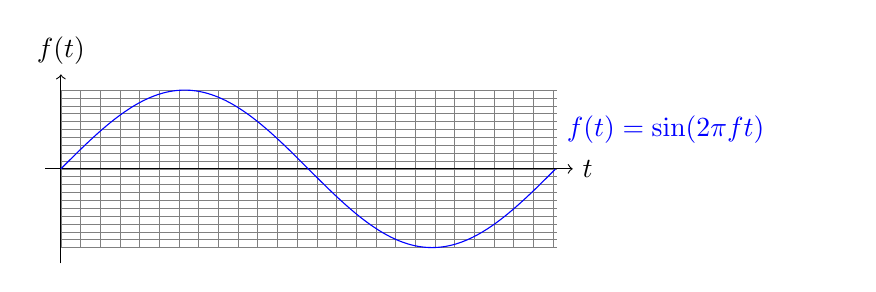
\begin{tikzpicture}[domain=0:6.28, samples=85,smooth]
			% Grundgrid
			%\draw<1>[style=help lines] (-0.1,-1.1) grid[xstep=1] (6.3,1.1);

			% 'ADC' Values
			\foreach \y in {-1,-0.9,...,1.1} { \draw<2>[style=help lines] (0,\y) -- (6.3,\y); }

			% Timesteps
			\foreach \x in {0,0.25,...,6.3} { \draw<3>[style=help lines] (\x,-1) -- (\x,1); }

			% Achsen
			\draw[->] (-0.2,0) -- (6.5,0) node[right] {$t$};
			\draw[->] (0,-1.2) -- (0,1.2) node[above] {$f(t)$};

			% Sinus
			\draw[color=blue] plot (\x,{sin(\x r)});
			\node[anchor=west,color=blue] (s1) at (6.3,0.5) {$f(t) = \sin (2 \pi f t)$};

			% Damit der Plot nicht rutscht
			\path (0,0) -- (10,0);
		\end{tikzpicture}
	\end{center}

	\begin{block}{Um das Signal digital zu verarbeiten, müssen wir}
		\begin{itemize}
			\item Amplitude
			\item und Zeit diskretisieren (``Abtastpunkte'' statt Verlauf)
		\end{itemize}
		Wie viele Abtastpunkte ($\Rightarrow$Speicherplatz) brauchen wir?
	\end{block}
\end{frame}

\begin{frame}[t]
	\frametitle{Ein Signal abtasten}
	\begin{center}
		% Sinus mit nur (etwas mehr als) 2 Samples/per einzeln einblenden:
		% höherfrequente Sinussignale die auch passen
		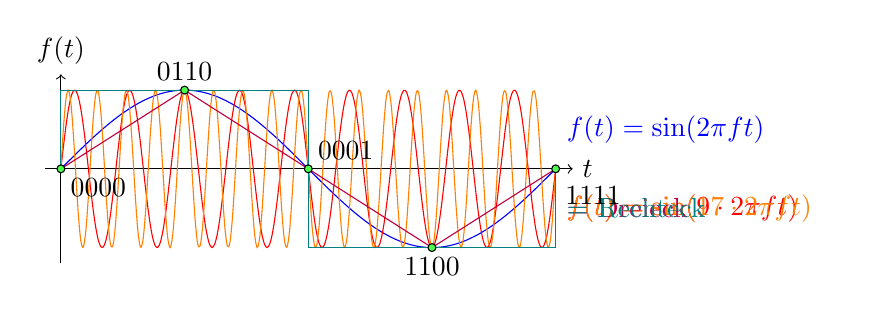
\begin{tikzpicture}[domain=0:6.28, samples=200,smooth]
			\tikzstyle{spt}=[color=black,fill=green!70]
			% Grid
%			\draw[style=help lines] (-0.1,-1.1) grid (6.3,1.1);

			% Achsen
			\draw[->] (-0.2,0) -- (6.5,0) node[right] {$t$};
			\draw[->] (0,-1.2) -- (0,1.2) node[above] {$f(t)$};

			% Grundsinus
			\draw[color=blue] plot (\x,{sin(\x r)});
			\node[anchor=west,color=blue] (s1) at (6.3,0.5) {$f(t) = \sin (2 \pi f t)$};

			% Vielfach-Sinuse
			%\draw[color=red] plot[id=v1\thecnt] (\x,{sin((#1) * (\x r) + (#2))}) node[below right]
			%	{$f(x) = \sin (#1 x)$};
			\draw<2>[color=red] plot (\x,{sin((9 * \x) r)});
			\node<2>[anchor=west,color=red] (s2) at (6.3,-0.5) {$f(t) = \sin (9 \cdot 2 \pi f t)$};

			\draw<3>[color=orange] plot (\x,{sin((17 * \x) r)});
			\node<3>[anchor=west,color=orange] (s3) at (6.3,-0.5) {$f(t) = \sin (17 \cdot 2 \pi f t)$};
			% Damit der Plot nicht rutscht
			\path (0,0) -- (10,0);

			\draw<4>[color=purple] (0,0) -- (pi/2,1) -- (pi,0) -- (3*pi/2,-1)
				-- (2*pi,0);
			\node<4>[anchor=west,color=purple] (t1) at (6.3,-0.5) {$=$ Dreieck};

			\draw<5>[color=teal] (0,0) -- (0,1) -- (pi,1) -- (pi, -1)
				-- (2*pi,-1) -- (2*pi,0);
			\node<5>[anchor=west,color=teal] (r1) at (6.3,-0.5) {$=$ Rechteck};

			% Abtastpunkte
			\draw[spt] (0,0) circle (0.05);
			\node<1>[anchor=north west] (ap1) at (0,0) {0000};

			\draw[spt] (pi/2,1) circle (0.05);
			\node<1>[anchor=south] (ap2) at (pi/2,1) {0110};

			\draw[spt] (pi,0) circle (0.05);
			\node<1>[anchor=south west] (ap3) at (pi,0) {0001};

			\draw[spt] (3*pi/2,-1) circle (0.05);
			\node<1>[anchor=north] (ap4) at (3*pi/2,-1) {1100};
			\path (3*pi/2,-1) -- +(0,-0.54);

			\draw[spt] (2*pi,0) circle (0.05);
			\node<1>[anchor=north west] (ap5) at (2*pi,-0.1) {1111};
		\end{tikzpicture}
	\end{center}

		\begin{block}{Kann ein Signal eindeutig rekonstruiert werden?}
			\uncover<2->{
				Es gibt unendlich viele Möglichkeiten ein abgetastetes Signal
				(falsch) zu rekonstruieren!
			}
		\end{block}
\end{frame}

\begin{frame}[t]
	\begin{center}
		% Robert's Signal aus 2 Sinussen: enmal als Summe, darunter die
		% einzelnen Komponenten, noch keine Abtastpunkte

		% Robert's Signal, diesmal mit zu wenigen Punkten
		%einblenden: passended niederfrequentes Signal
		%einblenden: mehr Punkte
		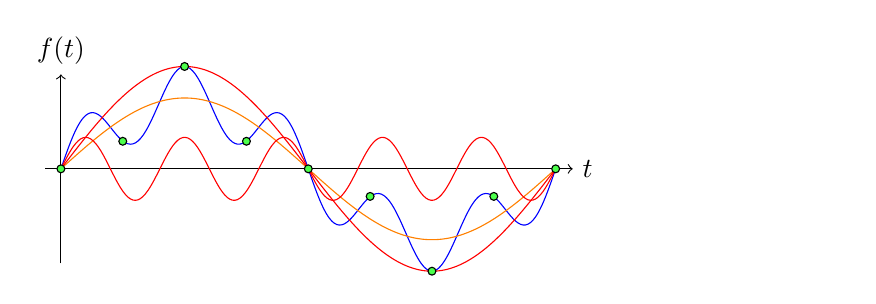
\begin{tikzpicture}[domain=0:6.28, samples=200,smooth]
			\tikzstyle{spt}=[color=black,fill=green!70]
			% Grid
%			\draw[style=help lines] (-0.1,-1.1) grid (6.3,1.1);

			% Achsen
			\draw[->] (-0.2,0) -- (6.5,0) node[right] {$t$};
			\draw[->] (0,-1.2) -- (0,1.2) node[above] {$f(t)$};

			% Überlagerung
			\draw[color=blue] plot (\x,{0.9 * sin(\x r) + 0.4 * sin((5 * \x) r)});

			% Grundsinus
			\draw<2>[color=orange] plot (\x,{0.9 * sin(\x r)});

			% Vielfach-Sinuse
			\draw<2>[color=red] plot (\x,{0.4 * sin((5 * \x) r)});

			% Simpler Match -- Nein, ich konstruiere mir meine Beispiele nicht
			% so einfach ;)
			\draw<4>[color=red] plot (\x, {1.3 * sin(\x r)});

			% Abtastpunkte
			\draw<3->[spt] (0,0) circle (0.05);
			\draw<3->[spt] (pi/2,1.3) circle (0.05);
			\draw<3->[spt] (pi,0) circle (0.05);
			\draw<3->[spt] (3*pi/2,-1.3) circle (0.05);
			\draw<3->[spt] (2*pi,0) circle (0.05);

			\draw<5->[spt] (pi/4  , 0.35) circle (0.05);
			\draw<5->[spt] (3*pi/4, 0.35) circle (0.05);
			\draw<5->[spt] (5*pi/4,-0.35) circle (0.05);
			\draw<5->[spt] (7*pi/4,-0.35) circle (0.05);

			% Damit der Plot nicht rutscht
			\path (0,0) -- (10,0);
			\path (0,0) -- (0,-1.36);

		\end{tikzpicture}
	\end{center}

	\only<2>{
		\begin{block}{Fourieranalyse:}
			\begin{itemize}
				\item Man kann jedes Signal als Summe von Sinussignalen
					darstellen.
			\end{itemize}
		\end{block}
	}
	\only<3-4>{
		\begin{block}{Wie viele Abtastpunkte brauchen wir mindestens?}
			\uncover<4->{
				Abtasttheorem: Wir brauchen zumindest 2 Abtastwerte pro
				Periode des höchstfrequenten Sinus.
			}
		\end{block}
	}
	\only<5>{
		\begin{block}{Vorgangsweise}
			\begin{itemize}
				\item Wir legen die höchste relevante Frequenz fest
					(Hörbereich \ldots).
				\item Wir filtern alle höheren Frequenzen weg (Tiefpass):\\
					Dadurch können wir bei der Rekonstruktion alle höheren
					Frequenzen ausschließen.
			\end{itemize}
		\end{block}
	}
\end{frame}

\begin{frame}
	\frametitle{Grenzen der Abstraktion}

	\begin{block}{Warum also Hintergründe verstehen, ``unter die Haube
			blicken''?}
		\begin{itemize}
			\item Interesse / Neugier?
			\item Um es ein bisschen besser machen zu können?
		\end{itemize}
	\end{block}

	\medskip

	\uncover<2->{
\begin{itemize}			
	\item Weil es auch jemanden geben muss, der die Abstraktion erstellt.
	\item	\alert<3>{Weil man Abstraktionen nur verwenden sollte, wenn man auch ihre
			Grenzen kennt!}
\end{itemize}
	}
	\medskip

	\begin{block}{Aber:}<4->
		Trifft man denn wirklich auf so komplizierte Spezialfälle wo
		Abstraktionen versagen?
	\end{block}
\end{frame}


\begin{frame}
	\frametitle{Abtasttheorem --- Ein praktisches Beispiel}

	\begin{block}{Der einsame Hirte}

		hat bei einer Spielzeit von 4:25 in unkomprimierter Form bei

		\begin{itemize}
			%Hörbeispiel; perfekter Kland
			\item<1-> Abtastung mit \SI{44100}{\hertz}: \SI{41}{\mega\byte}
				%shepherd
	%			\only<1>{
	%				\includemedia[
	%					addresource=media/shepherd_cut.mp3,
	%					flashvars={
	%						source=media/shepherd_cut.mp3&autoPlay=true
	%					}
	%				]{\fbox{Play}}{APlayer.swf}
	%			}
			%Hörbeispiel; akzeptabler Klang
			\item<2-> Abtastung mit \SI{22050}{\hertz}: \SI{21}{\mega\byte}
				%shepherd_filter_22050
	%			\only<2>{
	%				\includemedia[
	%					addresource=media/shepherd_filter_22050.mp3,
	%					flashvars={
	%						source=media/shepherd_filter_22050.mp3&autoPlay=true
	%					}
	%				]{\fbox{Play}}{APlayer.swf}
	%			}
			%Hörbeispiel; kacke Klang; fehlende Frequenzen
			\item<3-> Abtastung mit \phantom{2}\SI{2205}{\hertz}: \phantom{2}\SI{2.1}{\mega\byte}
				%shepherd_filter_2205
	%			\only<3>{
	%				\includemedia[
	%					addresource=media/shepherd_filter_2205.mp3,
	%					flashvars={
	%						source=media/shepherd_filter_2205.mp3&autoPlay=true
	%					}
	%				]{\fbox{Play}}{APlayer.swf}
	%			}
			%Hörbeispiel; kacke Klang; aliasing
			\item<4-> Abtastung mit \phantom{2}\SI{2205}{\hertz} ohne Filter: \SI{2.1}{\mega\byte}
				%shepherd_alias_2205
	%			\only<4>{
	%				\includemedia[
	%					addresource=media/shepherd_alias_2205.mp3,
	%					flashvars={
	%						source=media/shepherd_alias_2205.mp3&autoPlay=true
	%					}
	%				]{\fbox{Play}}{APlayer.swf}
	%			}

		\end{itemize}
	\end{block}

	\medskip

	\begin{block}{Die Abtastfrequenz macht's aus!}<5>
		Auch hier macht es Sinn die Theorie zu kennen!
	\end{block}
\end{frame}

